\subsection{\textbf{DER (Diagrama Entidade Relacionamento)}}

\noindent \cbox{
     Colocar aqui o DER do seu projeto. Ele pode ser elaborado em ferramentas de modelagem UML ou gerados pelo ambiente de desenvolvimento. (Deve existir em todos os projetos que envolvem banco de dados). O exemplo abaixo é para vocês lembrarem como é.
}
   
\begin{figure}[H]
    \centering
    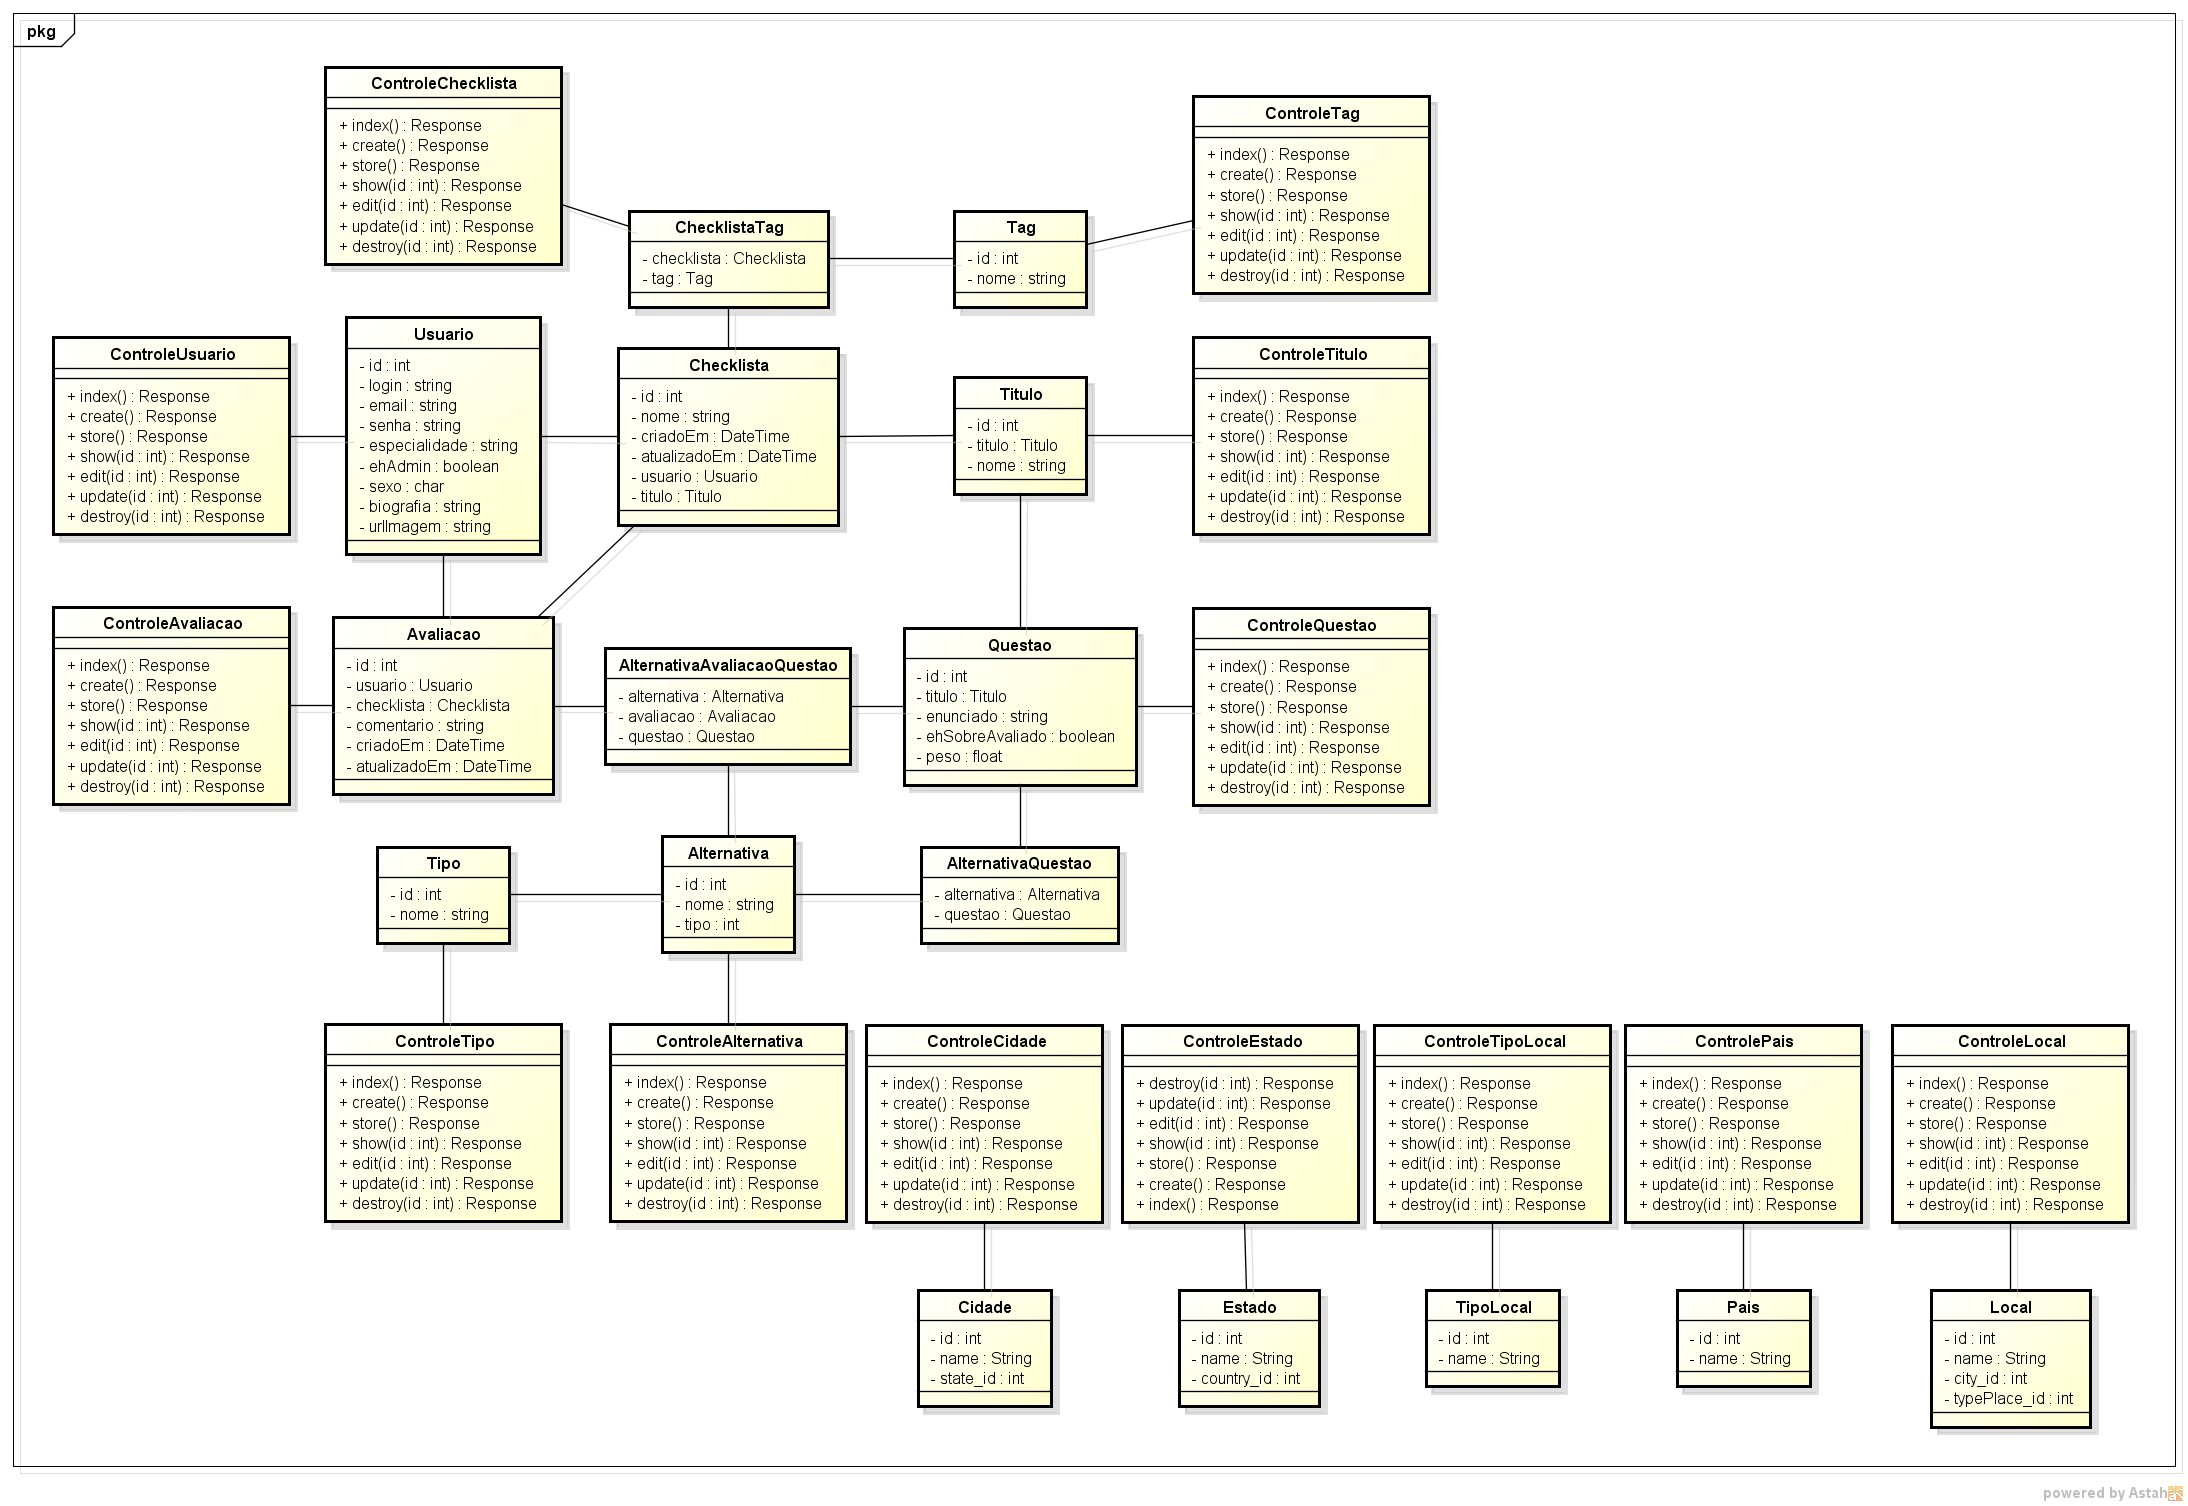
\includegraphics[scale=.3]{imgs/DER.png}
    \label{fig:my_label}
\end{figure}

